\documentclass[uplatex,a4paper,dvipdfmx,titlepage,oneside,openany]{jsarticle}
\pagestyle{empty}
\usepackage{amsmath,amsthm,amsfonts,latexsym,mathtools,bm,ulem,amssymb,tikz,circuitikz,graphicx}

\usepackage{times}
\usepackage[subrefformat=parens]{subcaption}
\usepackage{here}
\usepackage{siunitx}
\usepackage{physics}
\usepackage{upgreek}%ギリシャ文字を立てる
\usepackage{tikz-3dplot}
\begin{document}
	\begin{figure}
		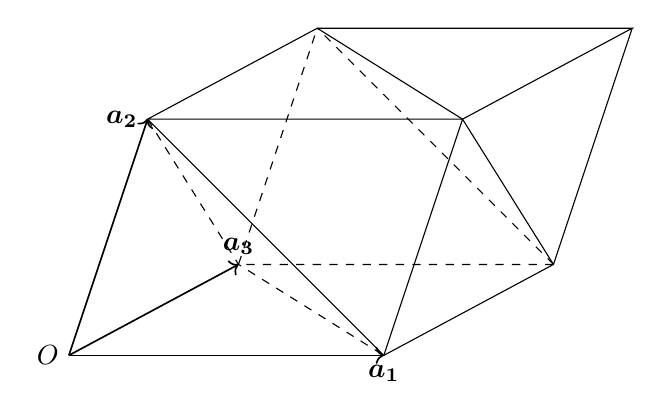
\begin{tikzpicture}
			\draw[->,semithick] (0,0,0) node[left]{$O$}--++(4,0,0) node[below]{$\bm{a_1}$};
			\draw[->,semithick] (0,0,0)--++(1,3,0) node[left]{$\bm{a_2}$};
			\draw[->,semithick] (0,0,0)--++(1,0,-3) node[above]{$\bm{a_3}$};
			\draw[] (4,0,0) --++(1,3,0)--++(-4,0,0)--++(1,0,-3)--++(4,0,0)--++(-1,0,3);
			\draw[] (4,0,0) --++(1,0,-3)--++(1,3,0);
			\draw[dashed] (5,0,-3)--++(-4,0,0)--++(1,3,0);
			\draw (4,0,0)--++(-3,3,0);3);
			\draw[dashed] (1,3,0)--++(0,-3,-3)--++(3,0,3);
			\draw (5,0,-3)--++(0,3,3)--++(-3,0,-3);
			\draw[dashed] (5,0,-3)--++(-3,3,0);
		\end{tikzpicture}
	\end{figure}
	\begin{figure}
		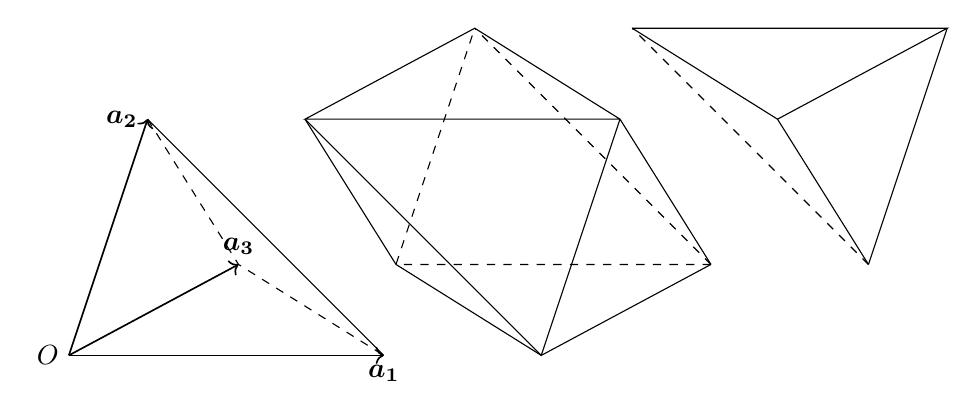
\begin{tikzpicture}
			\draw[->,semithick] (0,0,0) node[left]{$O$}--++(4,0,0) node[below]{$\bm{a_1}$};
			\draw[->,semithick] (0,0,0)--++(1,3,0) node[left]{$\bm{a_2}$};
			\draw[->,semithick] (0,0,0)--++(1,0,-3) node[above]{$\bm{a_3}$};
			\draw (4,0,0)--++(-3,3,0);
			\draw[dashed] (1,3,0)--++(0,-3,-3)--++(3,0,3);
			
			\draw[] (3,3,0)--++(0,-3,-3)--++(3,0,3)--++(1,3,0)--++(-4,0,0)--++(1,0,-3)--++(3,0,3)--++(0,-3,-3);
			\draw[] (6,0,0) --++(1,0,-3);
			\draw[dashed] (7,0,-3)--++(-3,3,0);
			\draw[] (6,0,0)--++(-3,3,0);
			\draw[dashed] (7,0,-3)--++(-4,0,0)--++(1,3,0);
			
			\draw (6,3,-3)--++(4,0,0)--++(-1,0,3);
			\draw (9,0,-3)--++(1,3,0);
			\draw (9,0,-3)--++(0,3,3)--++(-3,0,-3);
			\draw[dashed] (9,0,-3)--++(-3,3,0);
		\end{tikzpicture}
	\end{figure}
	\begin{figure}
		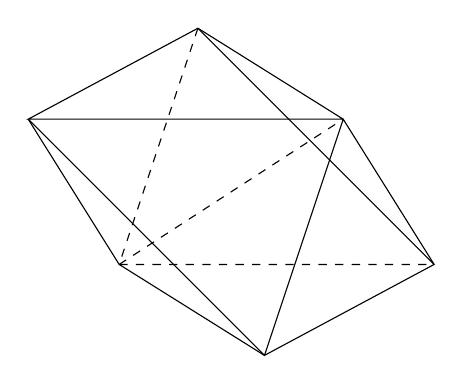
\begin{tikzpicture}
			\draw[] (3,3,0)--++(0,-3,-3)--++(3,0,3)--++(1,3,0)--++(-4,0,0)--++(1,0,-3)--++(3,0,3)--++(0,-3,-3);
			\draw[] (6,0,0) --++(1,0,-3)--++(-3,3,0);
			\draw[] (6,0,0)--++(-3,3,0);
			\draw[dashed] (4,3,-3)--++(-1,-3,0)--++(4,0,0);
			\draw[dashed] (3,0,-3)--++(4,3,3);
		\end{tikzpicture}
	\end{figure}
	\begin{figure}
		\begin{tikzpicture}
			\draw[] (3,3,0)--++(0,-3,-3)--++(3,0,3)--++(1,3,0)--++(-4,0,0)--++(1,0,-3)--++(3,0,3)--++(0,-3,-3);
			\draw[] (6,0,0) --++(1,0,-3);
			\draw[dashed] (7,0,-3)--++(-3,3,0);
			\draw[] (6,0,0)--++(-3,3,0);
			\draw[dashed] (4,3,-3)--++(-1,-3,0)--++(4,0,0);
			\draw[dashed] (3,0,-3)--++(4,3,3);
			
			\draw[->,thin] (1.5,1,-3)--++(-1,0,0);
			\draw (-1,3,-3)--++(-1,0,3)--++(4,0,0)--++(-3,0,-3);
			\draw (-2,3,0)--++(0,-3,-3)--++(4,3,3);
			\draw[dashed] (-1,3,-3)--++(-1,-3,0);
			
			\draw[->,thin] (6,-0.2,0)--++(0,-0.5,0);
			\draw (6,-4,0)--++(1,3,0)--++(-4,0,0)--++(3,-3,0)--++(-3,0,-3)--++(0,3,3);
			\draw[dashed] (7,-1,0)--++(-4,-3,-3);
			
			\draw[->,thin] (8,1.5,-1)--++(1,0,0);
			\draw (11,0,0)--++(1,0,-3)--++(0,3,3)--++(-1,-3,0)--++(-3,0,-3)--++(4,3,3);
			\draw[dashed] (12,0,-3)--++(-4,0,0);
			
			\draw[->,thin] (6.5,2.5,-2)--++(0.75,0.5,0);
			\draw (6,3,-3)--++(1,3,0)--++(3,0,3)--++(-4,-3,-3)--++(4,0,0)--++(0,3,3);
			\draw[dashed] (7,6,-3)--++(3,-3,0);
		\end{tikzpicture}
	\end{figure}
		
\end{document}